\documentclass[9pt,lineno]{elife}

% graphicx package, useful for including eps and pdf graphics
\usepackage{graphicx}
\DeclareGraphicsExtensions{.png,.png,.jpg}

% basic packages
\usepackage{color}
\usepackage{parskip}
\usepackage{float}
\usepackage{microtype}
\usepackage{url}
\usepackage{hyperref}
\usepackage{booktabs}
\usepackage{makecell}
\usepackage{multirow}

% text layout
\usepackage{geometry}
\geometry{textwidth=17cm} % 15.25cm for single-space, 16.25cm for double-space
\geometry{textheight=22.5cm} % 22cm for single-space, 22.5cm for double-space

% helps to keep figures from being orphaned on a page by themselves
\renewcommand{\topfraction}{0.85}
\renewcommand{\textfraction}{0.1}

% bold the 'Figure #' in the caption and separate it with a period
% Captions will be left justified
\usepackage[labelfont=bf,labelsep=period,font=small]{caption}

% cite package, to clean up citations in the main text. Do not remove.
%\usepackage{cite}
%\usepackage{natbib}

%% \usepackage{lineno}
%% \linenumbers

\usepackage{authblk}
\renewcommand\Authands{ \& }
\renewcommand\Authfont{\normalsize \bf}
\renewcommand\Affilfont{\small \normalfont}
\makeatletter
\renewcommand\AB@affilsepx{, \protect\Affilfont}
\makeatother

% latexdiff

%DIF UNDERLINE PREAMBLE %DIF PREAMBLE
\RequirePackage[normalem]{ulem} %DIF PREAMBLE
\RequirePackage{color}\definecolor{RED}{rgb}{1,0,0}\definecolor{BLUE}{rgb}{0,0,1} %DIF PREAMBLE
\providecommand{\DIFadd}[1]{{\protect\color{blue}\uwave{#1}}} %DIF PREAMBLE
\providecommand{\DIFdel}[1]{{\protect\color{red}\sout{#1}}}                      %DIF PREAMBLE
%DIF SAFE PREAMBLE %DIF PREAMBLE
\providecommand{\DIFaddbegin}{} %DIF PREAMBLE
\providecommand{\DIFaddend}{} %DIF PREAMBLE
\providecommand{\DIFdelbegin}{} %DIF PREAMBLE
\providecommand{\DIFdelend}{} %DIF PREAMBLE
%DIF FLOATSAFE PREAMBLE %DIF PREAMBLE
\providecommand{\DIFaddFL}[1]{\DIFadd{#1}} %DIF PREAMBLE
\providecommand{\DIFdelFL}[1]{\DIFdel{#1}} %DIF PREAMBLE
\providecommand{\DIFaddbeginFL}{} %DIF PREAMBLE
\providecommand{\DIFaddendFL}{} %DIF PREAMBLE
\providecommand{\DIFdelbeginFL}{} %DIF PREAMBLE
\providecommand{\DIFdelendFL}{} %DIF PREAMBLE

% comments
%% \definecolor{purple}{rgb}{0.459,0.109,0.538}
%% \def\tbc#1{\textcolor{purple}{[#1]}}
%% \def\rnc#1{\textcolor{blue}{[#1]}}
%% \def\jhc#1{\textcolor{green}{[#1]}}

\title{Genetic cartography reveals ancestral relationships of human pathogenic viruses}

\author[1]{Sravani Nanduri}
\author[2]{John Huddleston}
\author[2]{Allison Black}
\author[2*]{Trevor Bedford}

\affil[1]{Issaquah High School, Issaquah, WA, USA}
\affil[2]{Vaccine and Infectious Disease Division, Fred Hutchinson Cancer Research Center, Seattle, WA, USA}

\corr{trevor@bedford.io}{TB}

\date{}

\begin{document}
\maketitle

\begin{abstract}
\end{abstract}

\section*{Introduction}

Tracking the evolution of human pathogenic viruses in real time enables epidemiologists to respond quickly to emerging epidemics and local outbreaks.
Real-time analyses of viral evolution typically rely on phylogenetic methods.
These methods can reconstruct the evolutionary history of viral populations from viral genome sequences and estimate states of inferred ancestral viruses including their most likely genome sequence, time of circulation, and geographic location (gen epi papers).
Importantly, these methods assume that all sequence data share an evolutionary history represented by the clonal replication of genomes.
In practice, the evolutionary histories of many human pathogenic viruses including seasonal influenza viruses, Zika virus, and coronaviruses violate this assumption through processes of recombination or reassortment.
Researchers have attempted to compensate for these evolutionary mechanisms by limiting their analyses to specific genes (citation?), concatenating multiple genes despite their different evolutionary histories (citation?), or developing more sophisticated models to represent the joint likelihoods of multiple co-evolving lineages represented by networks rather than trees (Muller).
However, several key questions in genomic epidemiology do not require full phylogenetic inference of ancestral relationships and states.
For example, genomic epidemiologists commonly need to 1) identify clusters of closely related genomes that represent regional outbreaks or new variants of concern (Black et al.? MicrobeTrace?), 2) rapidly place newly sequenced viral genomes in the evolutionary context of other circulating strains (USHER, NextClade), and 3) flag low-quality or mislabeled genome sequences for exclusion from their analyses.
These common use cases can all be addressed by standard statistical methods including clustering, classification, and outlier detection.
These methods make few assumptions about the input data and should be therefore applicable to genomic data that violate phylogenetic assumptions.

To apply these methods to a population of viral genomes, we need metrics to compare genome sequences to each other and algorithms to reduce the highly multidimensional input data (M x N for M genomes of length N) to one or two dimensions where clustering, classification, and outlier detection are more tractable.
The number of mismatches between any pair of aligned genome sequences, also known as the Hamming distance, provides a natural distance metric for viral genomes.
Indeed, most phylogenetic methods start by building a matrix of Hamming distances between all sequences in a given multiple sequence alignment.
Many dimensionality reduction algorithms including multidimensional scaling (MDS), t-SNE, and UMAP accept such distance matrices as an input and produce a corresponding lower-dimensional representation or “embedding” of those data.
Alternately, principal components analysis (PCA) only requires the input data to be transformed to a matrix of integers before it can embed those data into a few orthogonal dimensions.

Each of these embedding methods has been applied to genomic data to visualize relationships between individuals and identify clusters of related genomes.
PCA has been applied to single nucleotide polymorphisms (SNPs) of human genomes (Novembre 2008, McVean 2009, Auton et al. 2015) and to multiple sequence alignments of viral genomes (Metsky et al. 2017).
Although PCA is a generic linear algebra algorithm that optimizes for an orthogonal embedding of the data, the principal components from SNPs represent mean coalescent times and therefore recapitulate broad phylogenetic relationships (McVean 2009).
MDS has been applied to multiple gene segments of seasonal influenza viruses to understand evolutionary relationships between segments (Rambaut et al. 2008).
MDS attempts to embed input data into a lower dimensional representation such that each pair of data points are as far apart in the embedding as they are in the original data.
More modern embedding methods like t-SNE and UMAP have also been applied to SNPs from human genomes (Diaz-Papkovich et al. 2019) and single-cell transcriptomes ([Becht et al. 2018](https://www.nature.com/articles/nbt.4314), [Kobak and Berens 2019](https://www.nature.com/articles/s41467-019-13056-x)) .
t-SNE and UMAP build on manifold learning methods like MDS to find low-dimensional embeddings of data that place similar points close together and dissimilar points far apart ([Kobak and Linderman 2021](https://www.nature.com/articles/s41587-020-00809-z)).

Although these embedding methods have been used to investigate relationships in populations of genomes, there has been no systematic assessment of their respective accuracies when applied to human pathogenic viruses.
To this end, we applied PCA, MDS, t-SNE, and UMAP to four human viruses including seasonal influenza virus A/H3N2, Zika virus, MERS-CoV, and SARS-CoV-2.
For each of the resulting embeddings, we quantified the relationship between genetic and Euclidean distances in the embedding space and the degree to which clusters in the embedding recapitulated previously defined phylogenetic clades.
These results inform recommendations for which embedding methods and parameters to use to answer specific questions relevant to genomic epidemiology.

\section*{Results}

\subsection*{Seasonal influenza A/H3N2}

\begin{figure}[htb]
  \begin{center}
  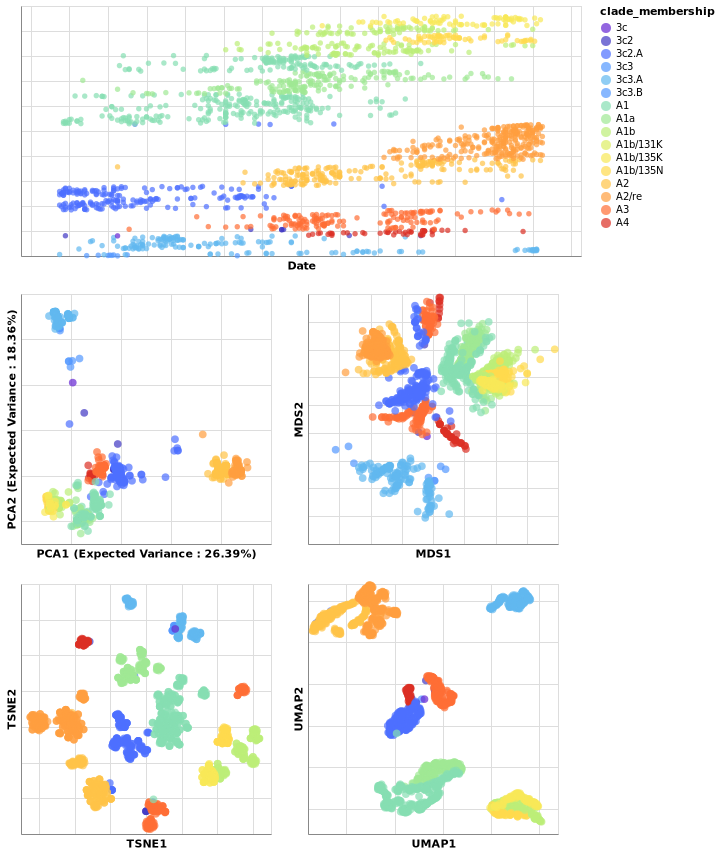
\includegraphics[width=\columnwidth]{flu-embeddings}
  \caption{
  }
  \label{fig:seasonal-influenza-h3n2-ha-embeddings}
  \end{center}
\end{figure}

\section*{Discussion}

\section*{Materials and methods}

\subsection*{Data and software availability}

The entire workflow for our analyses was implemented with Snakemake \citep{Snakemake}.
We have provided all source code, configuration files, and datasets at \href{https://github.com/blab/cartography}{https://github.com/blab/cartography}.

\section*{Acknowledgments}

\section*{Author contributions}

SN...
JH...
AB...
TB...

\section*{Competing interests}

The authors declare that no competing interests exist.

\section*{Supplemental Files}

\bibliography{cartography}

\end{document}
